\documentclass[12pt]{article}

% Packages for double-spacing
\usepackage{setspace}
\usepackage{graphicx}
\usepackage{mathbbol}
\doublespacing
\boldmath

\begin{document}

% Title and author information
\title{The Graph Neural Network Model}

\maketitle

% Abstract
\begin{abstract}
    A remarkable number of ideas across various domains can be effectively
    depicted as graphs, ranging from social networks and railway maps to
    molecules. Graphs offer an elegant way to abstract these concepts, making
    them a primary tool for representing data. This abstraction not only
    highlights the characteristics of individual data points but also captures
    the relationships between them. However, this versatility poses a challenge
    in the field of machine learning, as desining algorithms that efficiently
    handle such interconnected data has proven to be a challenging task.
\end{abstract}

% Introduction
\section{Introduction}
      We  shall  start  by  giving a brief introduction to out mathematical model. A
    graph  $G$  is  a  pair  $(V,  E)$,  where  $V$  is  the set of vertices, and $E
    \subseteq  V  \times  V$  is  the  set  of edges, representing the relationships
    between  the  vertices.  An  example  of  a  graph would be a railway map, where
    the  vertices  are  the  stations  and  the  edges  are  the railways connecting
    them.  Often  we're  interested  in  giving some attributes to the edges. In the
    case  of  the  railway  map,  we  could  assign the length of the railway to the
    edges,  in  which  case  the graph would be a weighted graph. On the other hand,
    edges   could   be  multidemensional,  in  which  case  the  graph  would  be  a
    hypergraph,  which  is  especially  useful for representing molecules, where the
    vertices are the atoms and the edges are the bonds between them.

     \begin{figure}[h]
         \centering
         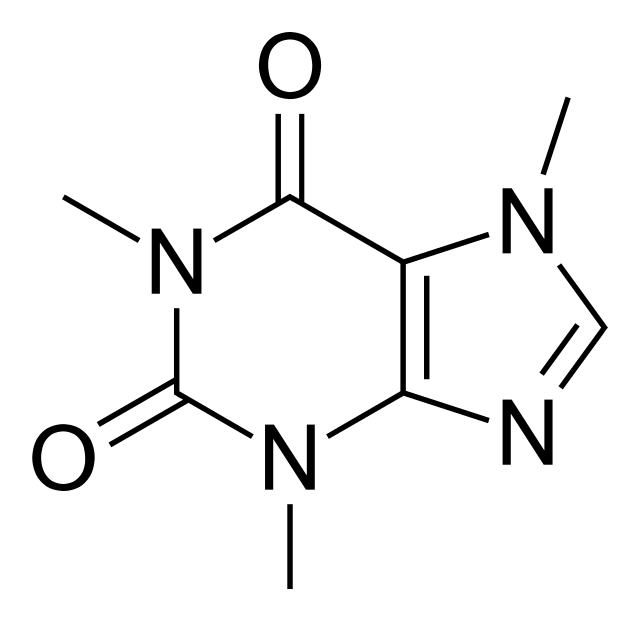
\includegraphics[width=0.4\textwidth]{img/Caffeine_structure.png}
           \caption{A   molecule   of  caffeine,  represented  as  a  graph,  where  the
        vertices are the atoms and the edges are the bonds between them.}
         \label{fig:graph}
     \end{figure}
    
    While providing the definitions, we will stick to unweighted and undirected, i.e.
    simple,  graphs.  The model can be easily extended to other cases.
    For a vertex $v \in V$, the set $N(v) = \{u \in V | (u, v) \in E\}$ is called the
    neighborhood  of  $v$, while $E(v) = \{(u, v) \in E\}$. The  degree  of  a  vertex  $v$  is  $|N(v)|$,  i.e. the
    number  of  vertices  adjacent  to  $v$.
    \\

    For any meaningful application of graphs in data science and machine learning, we
    shall assign labels (real vectors) to the vertices and the edges. They will be represented by
    $l_v \in \mathbb{R}^{l_V}$ and $l_{(v, u)} \in \mathbb{R}^{l_E}$, respectively.

    

% Methodology
\section{The Graph Neural Network Model}
    \indent 
    In this section, we will present the Graph Neural Network model, which is a
    powerful algorithm for learning on graphs, first introduced by Scarselli et al.
    \cite{scarselli2009graph}. 
    \\
    \indent The novelty of the model lies in the fact that it is able to learn the relationships
    between the vertices of a graph, as the representation of each vertex depends on the
    representations of its neighbors.

    More formally, assume we are given a dataset of graphs: \\ $\mathcal{D} = \{(G_i, v_{i, j}, t_{i, j}) | G_i = (V_i, E_i), v_{i, j} \in V_i, t_{i, j} \in \mathbb{R}^m\}$, \\
    where $v_{i, j}$ is the $j$-th vertex of the $i$-th graph, and $t_{i, j}$ is the target label of $v_{i, j}$.
    The objective is to learn a function $\varphi : G \times V \rightarrow \mathbb{R}^m$ such that $\varphi(G_i, v_{i, j}) \approx t_{i, j}$,
    where $G$ and $V$ are the set of all graphs and vertices, respectively, considered in $\mathcal{D}$.
    \\
    \indent The underlying intuitive idea of this algorithm is that in a graph, vertices are representing object, data points, etc.,
    while the edges are representing the relationships between them. Therefore, the representation of a vertex should depend on the
    representations of its neighbors. To mimic this, we will attach a \textbf{\textit{state}} to each vertex, 
    $x_v \in \mathbb{R}^s$, which is encodes information contained in $N(v)$, and is used to compute an 
    \textbf{\textit{output}} $o_v \in \mathbb{R}^m$, s.t. $o_v \approx t_v$.
    \\
    \indent It is natural to express the dependence of $x_v$ on its neighbors as a function, so let 
    $f_w$ be a parametric function, called \textbf{\textit{local transition function}}.
    Similarly, let $g_w$ be the \textbf{\textit{local output function}}. Then, the state and output of a vertex $v$ are computed as follows:
    \begin{equation}
        x_v = f_w(l_v, l_{N(v)}, l_{E(v)}, x_{N(v)})
    \end{equation}
    \begin{equation}
        o_v = g_w(x_v, l_v)
    \end{equation}
    , where $l_v$, $l_{N(v)}$, $l_{E(v)}$ are the labels of $v$, $N(v)$, $E(v)$, respectively, stacked together,
    and $x_{N(v)}$ the states of the neighbors of $v$, stacked.

    \begin{figure}[t]
        \centering
        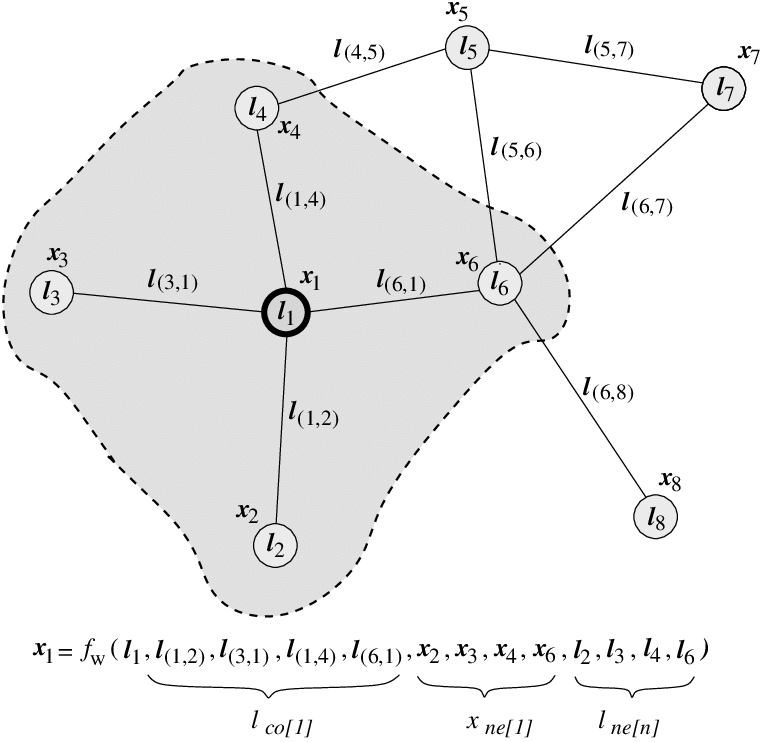
\includegraphics[width=0.7\textwidth]{img/A-graph-and-the-neighborhood-of-a-node-The-state-x-1-of-node-1-depends-on-the.png}
        \caption{A graph and the neighborhood of a node. The state $x_1$ of node 1 depends on the states of its neighbors, $x_2$, $x_3$, $x_4$, and $x_6$.}
        \label{fig:local_functions}
    \end{figure}

    \indent It is worth noting, nevertheless, that the use of $l_{N(v)}$ and $l_{E(v)}$ may be considered redundant,
    as $x_{N(v)}$ already encodes this information, while $l_v$ is contained in $x_v$ for $g_w$. This would be just a similar
    definition to $f_w$ and $g_w$.
    \\
    \indent Let $x$, $o$, $l_V$, and $l_E$ be the vectors constructed by stacking $x_v$, $o_v$, $l_v$, and $l_{(v, u)}$ respectively, for all $v \in V$
    and $(v, u) \in E$.
    Then, (1) and (2) can be rewritten as:
    \begin{equation}
        x = F_w(x, l_V, l_E)
    \end{equation}
    \begin{equation}
        o = G_w(x, l_V)
    \end{equation}
    , and we therefore call $F_w$ and $G_w$ the \textbf{\textit{global transition function}} and \textbf{\textit{global output function}}, respectively.
    \\
    \indent Naturally, we are only interested in the cases when $o$, and therefore $x$, are uniquelly defined, so that $\varphi$
    is indeed a function. While it is obvious that any feed-forward neural network satisfies this condition for $G_w$, it isn't
    by far the case for $F_w$, because of its recursive nature. Nevertheless, the Banach fixed-point theorem guarantees us that
    a uniquelly defined $x$ can be achieved, provided that $F_w$ is a contraction mapping, i.e. 
    $\exists \mu \in [0, 1) \forall x, y \in \mathbb{R}^s : ||F_w(x) - F_w(y)|| \leq \mu ||x - y||$. [reference to be inserted here, so far it is Wikipedia :-)]
    \\
    \indent The Banach fixed-point theorem also conveniently provides us with an iterative algorithm for 
    computing $x$, which converges exponentially fast for any $x(0) \in \mathbb{R}^s$:
    \begin{equation}
        x(t + 1) = F_w(x(t), l_V, l_E)
    \end{equation}
    , where $x(t)$ is the state of the vertices at the $t$-th iteration, and $x(0)$ is $l_V$ (my understanding, it is actually never mentioned in the paper what precisely is $x(0)$).
    Also I believe we can have yet another function, $H_w$ (which would be a straightforward MLP) that computes $x(0)$ in one step, namely $x = H_w(l_V, l_E)$, i.e. would map the labels to a higher-dimensional space. I'll experiment with this once I have the basic model working. 

    \begin{figure}[h]
        \centering
        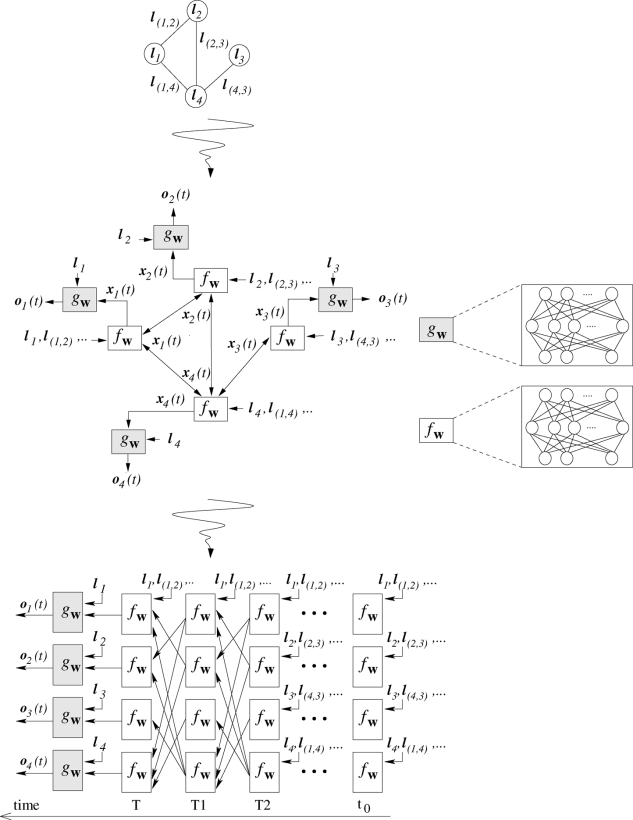
\includegraphics[width=0.9\textwidth]{img/An-illustration-of-the-iterative-process-of-the-GNN-model-The-state-of-each-node.png}
        \caption{An illustration of the iterative process of the GNN model. The state of each node is computed by the local transition function $f_w$ using the states of its neighbors.}
        \label{fig:iterative_process}
    \end{figure}

    Thus, the model behaves as follows:
    \begin{enumerate}
        \item The labels of the vertices and edges are mapped to a higher-dimensional space by $H_w$. (hypothesis / optional). Otwerwise, $x(0) = l_V$.
        \item The states of the vertices are computed iteratively by $F_w$, until convergence. Namely, for the time step $t+1$, we take for each vertex $v$ its state at the time step $t$, and the states of its neighbors at the time step $t$, $x_v(t)$, and of its neighbors, $x_{N(v)}(t)$, and compute $x_v(t+1) = f_w(x_v(t), x_{N(v)}(t))$. At any given time step. $f_w$ is applied simulataniously to all vertices.
        \item Repeat the previous step until convergence. I.e. for a hyperparameter $\epsilon > 0$, stop when $||x(t+1) - x(t)|| < \epsilon$. Let $x$ be the resulting, final state.
        \item Compute the output of each vertex by $G_w$, i.e. $o_v = g_w(x_v, l_v)$.
        \item Update the parameters of $F_w$, $G_w$, and $H_w$ by backpropagation.
    \end{enumerate}

\section{Backpropagation}
    

% Results
\section{Results}
This is the results section of your article.

% Conclusion
\section{Conclusion}
This is the conclusion section of your article.

% References
\begin{thebibliography}{9}
\bibitem{scarselli2009graph}
Scarselli, F., Gori, M., Tsoi, A. C., Hagenbuchner, M., \& Monfardini, G. (2009). The graph neural network model. IEEE Transactions on Neural Networks, 20(1), 61-80.

\end{thebibliography}

\end{document}




